\clearpage
\subsection{Procedure} % (fold)
\label{sub:procedure}

The computer is unintelligent, so performing anything meaningful requires a large number of instructions. Coding all of these directly in the program would be slow and time consuming. To avoid this programming languages offer the capability to group the instructions to perform a task into a \textbf{procedure}. 

A procedure is a list of instructions that gets the computer to perform a specific task. When a procedure is called it gets control of the computer and instructs it to perform the steps needed. Often these steps require data, so the procedure may need to be passed data when it is called. When the procedure finishes its task, control returns back to the code that called the procedure.

\begin{figure}[h]
   \centering
   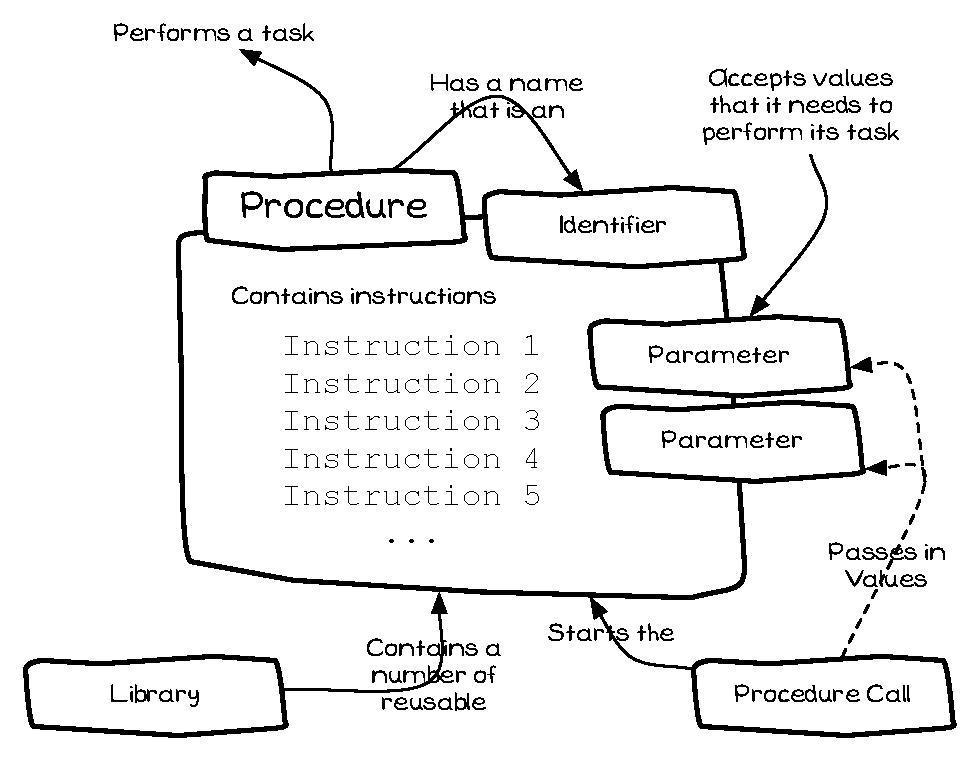
\includegraphics[width=0.9\textwidth]{./topics/program-creation/diagrams/Procedure} 
   \caption{A procedure contains instructions to perform a task, and may need to be passed data in order to do this}
   \label{fig:program-creation-procedure}
\end{figure}


\mynote{
\begin{itemize}
  \item A procedure is an \textbf{artefact}, something that can be created in code. 
  \item Figure \ref{fig:program-creation-procedure} shows the concepts related to procedures.
  \item A procedure is a programming artefact that can be called to perform a certain task.
  \item The name of a procedure is an \nameref{sub:identifier}.
  \item Each \nameref{sub:library} will contain a number of procedures to perform common tasks.
  \item The standard library will include procedures to write values to the Terminal.
  \item The SwinGame libraries contain procedures that can draw images on the screen, play sounds, and perform other tasks needed to create small games.
  \item Procedures are also known as \textbf{subroutines}, \textbf{sub-programs}, \textbf{methods} or \textbf{sub-procedures}.
\end{itemize}
}

% section program (end)